\chapter{Analysis} \label{cha:Analysis} \glsresetall
In this chapter every subcomponent will be part of an experiment in isolation to validate their function. Also, various test setups will be discussed for the purpose of making multi-module experiments in the AFE and control system to evaluate their performance and compatibility. As such, each module will be tested independently to validate its function before a larger, more comprehensive experiment is conducted. All figures in this chapter show measurements performed on physical hardware.

\section{Module Testing}
\subsection{Control System}
First, a bitstream was generated with a Pwm generator and AXI interconnect registers. An AXI interconnect register is a method to create GPIO interfaces between the logical processor and the Arm processor on the Zynq 7000 SoC using registers that temporarily store GPIO data in the bitstream overlay. A block diagram of the overlay can be seen in \cref{fig:app_fpga_block_diagram} and the JupyterLab notebook can be seen in \cref{fig:app_jupyter_notebook}.

\begin{figure}[htbp]
	\centering
	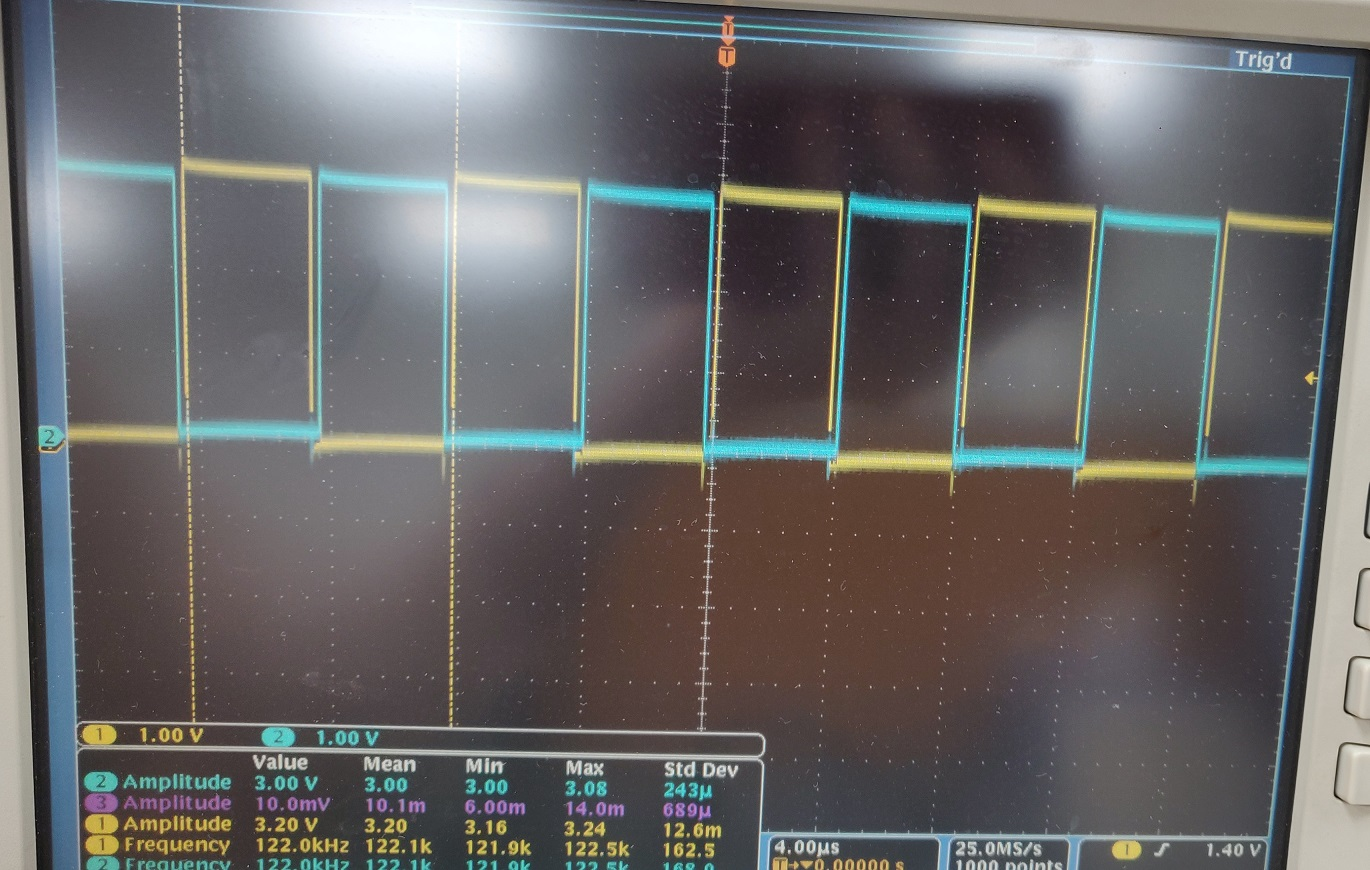
\includegraphics[width=.8\textwidth]{Figures/4_controlsystem_fpga_pwm.png}
	\caption{Complementary PWM output with Pynq Z1 FPGA and JupyterLab notebook}
	\label{fig:4_controlsystem_fpga_pwm}
\end{figure}
A preliminary implementation was implemented in Vivado and JupyterLab for a continuous complementary PWM controller. The resulting measurement can be seen in \cref{fig:4_controlsystem_fpga_pwm} before a clock configuration, which means the frequency corresponded to an arbitrary temporary pulse frequency of \qty{122}{\kilo\hertz}. As the initial test proved successful, the continued development and maturation of the pulser enabled a complete signal generator for the ultrasound pulse generator.

\begin{figure}[htbp]
	\centering
	\includegraphics[width=\linewidth]{Figures/5_controlsystem_fpga_pulser_logic.eps}
	\caption{Captured timing diagram of the control system pulser}
	\label{fig:5_controlsystem_pulser_logic}
\end{figure}
Seen in \cref{fig:5_controlsystem_pulser_logic} are the measured signals from the pulse generator showing the various timings of each signal captured with a Salae Logic Analyzer Pro 8. In the figure, there is observed a continuous \qty{20}{\mega\hertz} \texttt{CLK} signal for the demodulator. For \texttt{PRF}, the signal sets the ultrasound switch to transmit with a corresponding startdelay to the complementary \texttt{PWM} and \texttt{PWMN} pulses. To see a further explanation of each signal and its function, refer to \cref{fig:3_pulsegenerator_signal_block_diagram}.

\subsection{Power Stage}
An experiment is conducted to validate the function of the power stage. Using the jumpers, the PCB is configured without its onboard load, and a \gls{pzt} transducer is attached with a splitter adapter to connect the other side to an oscilloscope for data acquisition. Seen in \cref{fig:4_transmitter_meas} are actual measured inputs and outputs of the power stage. On the input, there are two complementary \qty{5}{\mega\hertz} signals with varying duty cycle to generate the desired dead time. On the output, we see the rail-to-rail push-pull operation of the \gls{mosfet} half-bridge. The schematic of the transmitter can be found in the appendix in \cref{fig:appendix_md1213db1}. Noticeable noise is observed in the input signal top and base but is negligible for successful operation. Possibly, the noise is due to a cable and adapter setup.
\begin{figure}[htbp]
	\centering
	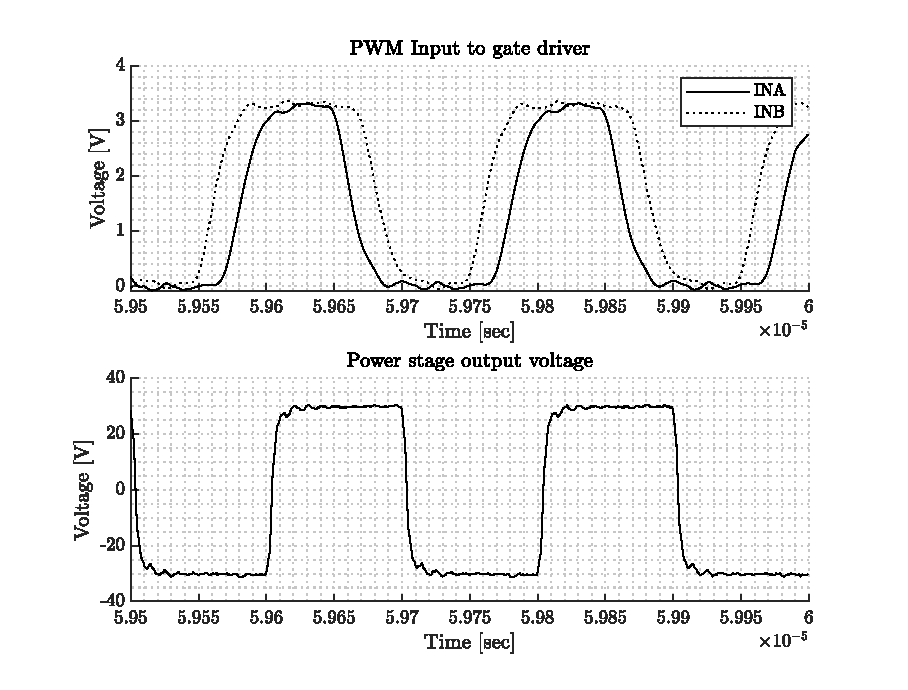
\includegraphics[width=.8\textwidth]{Figures/4_transmitter_pcb_out.eps}
	\caption[Measured input and output of power stage PCB]{Measured input and output of power stage PCB. (Above) Input to gate driver with dead-time (Below) Output of MOSFET half-bridge and the voltage across the load}
	\label{fig:4_transmitter_meas}
\end{figure}

\subsection{Transmit/Receive Switch}
\begin{figure}[htbp]
	\centering
	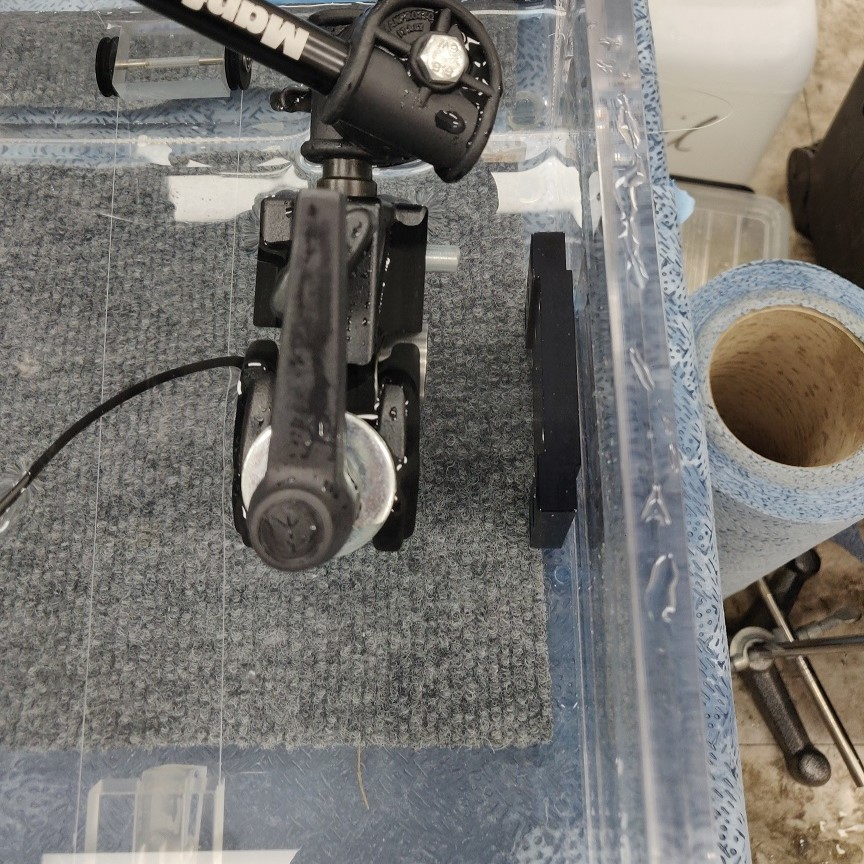
\includegraphics[width=.8\textwidth]{Figures/4_switch_meas_pic.jpg}
	\caption{TX/RX Switch reflection experiment with water tank}
	\label{fig:4_switch_meas_pic}
\end{figure}
For validating the TX/RX switch, an experiment is conducted with a \gls{pzt} transducer, water tank, function generator and an oscilloscope. Using two input signals, $f_{\mathrm{prf}}=\qty{10}{\kilo\hertz}$ switch signal, and $f_{0}=\qty{5}{\mega\hertz}$ burst mode transmit signal, the switch is configured to transmit and receive. A picture of the submerged transducer with a reflector can be seen in \cref{fig:4_switch_meas_pic}. After submerging the transducer in distilled water and measuring on the receiver side of the TX/RX switch, a reflected signal from the tank can be observed in \cref{fig:4_txrx_meas}.
\begin{figure}[htbp]
	\centering
	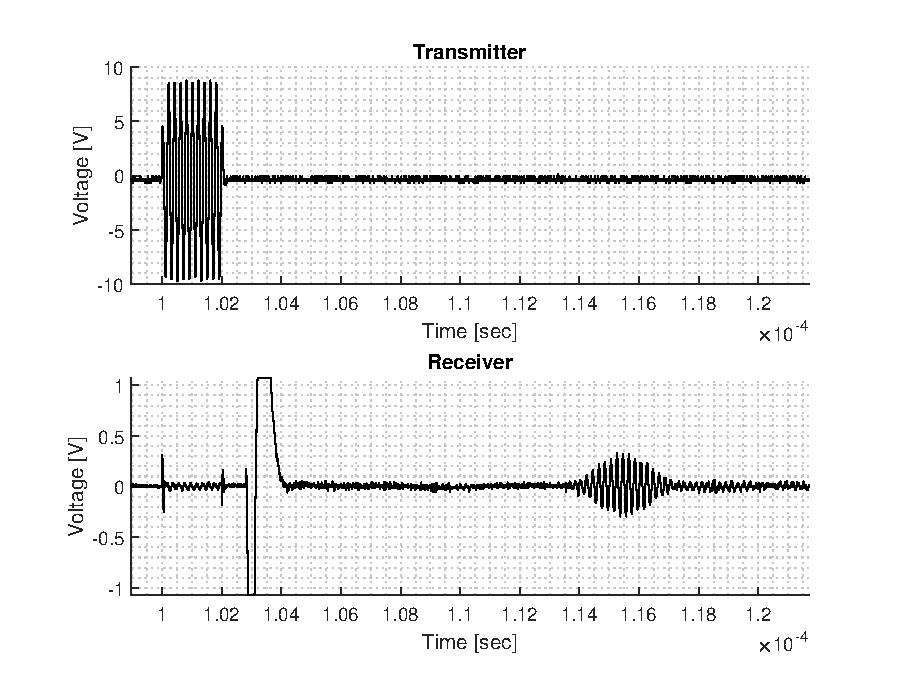
\includegraphics[width=.8\textwidth]{Figures/4_switch_pcb_meas.eps}
	\caption[Measured transmit and receive on Transmit/Receive Switch PCB]{Measured transmit and receive on Transmit/Receive Switch PCB (Above) Measured transmit voltage (Below) Received reflected signal off water tank}
	\label{fig:4_txrx_meas}
\end{figure}

\subsection{Band-pass Filter}
it is desired to validate its frequency response to determine if it functions as desired. To obtain the frequency response, a bode plot of the magnitude and phase is measured from \qty{300}{\kilo\hertz} until \qty{20}{\mega\hertz} using a \gls{vna} in a S21 configuration, meaning a measurement of the output in respect to the input. This measurement determines the difference in magnitude and phase of the output in comparison with the input signal. Observed in \cref{fig:4_bpf_measurement} is the frequency response of the band-pass filter measured on a \gls{vna}. It is noted that the pass band frequencies are mostly as expected with \qty{-0.5}{\decibel} frequencies at \qty{1.5}{\mega\hertz} and \qty{7}{\mega\hertz}. Though, the roll-off in the higher stop band appears somewhat lower than in the lower stop band. That would mean that it is plausible that higher frequency noise components are retained in the output than in the lower stop band. For the phase, it seems to have a significant phase delay, going from around \qty{100}{\degree} to \qty{250}{\degree} from the start to the end of the pass band.
\begin{figure}[htbp]
	\centering
	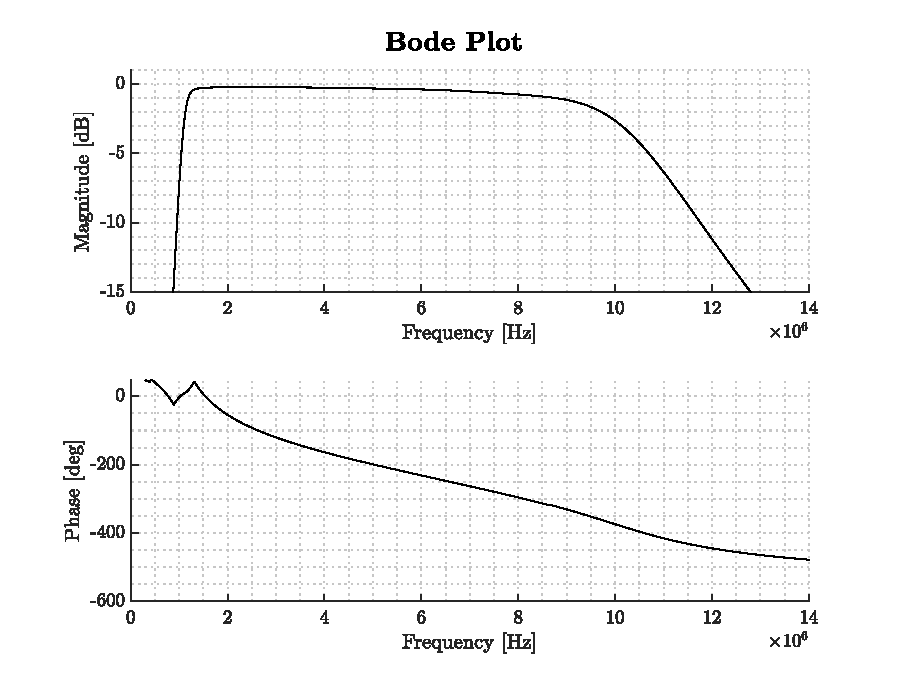
\includegraphics[width=.8\textwidth]{Figures/4_bpf_measurement_vna.eps}
	\caption[Band-pass filter bode plot]{Band-pass Filter bode plot from \qtyrange{0.3}{14}{\mega\hertz} with (above) magnitude and (below) phase}
	\label{fig:4_bpf_measurement}
\end{figure}

\subsection{Preamplifier}
Seen in \cref{fig:4_preamp_in} are measurements of the preamplifier circuits showing a \qty{70}{\milli\volt} input signal and a \qty{300}{\milli\volt} output signal with a \qty{2.5}{\volt} DC bias. In this application, however, only the \gls{lna} is used, and the \gls{vga} is bypassed in the hardware preamplifier configuration. The schematic of the preamplifier circuit is part of the demodulation schematic and can be found in the appendix in \cref{fig:appendix_ad8333}.
\begin{figure}[htbp]
	\centering
	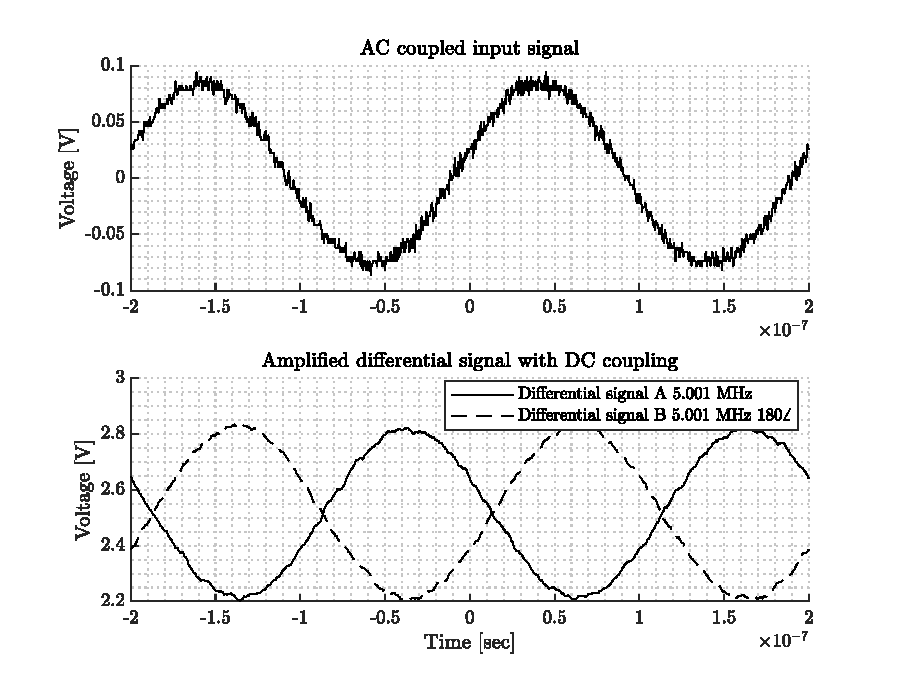
\includegraphics[width=.8\textwidth]{Figures/4_preamplifier_pcb.eps}
	\caption[Measured input and output of preamplifier PCB]{Measured input of preamplifier PCB, (Above) AC coupled input signal with amplitude \qty{1}{\volt} (Below Measured output of preamplifier PCB, Differential signal with DC coupling and $\times \qty{19}{\decibel}$ amplification)}
	\label{fig:4_preamp_in}
\end{figure}

\subsection{Demodulator}
An experiment is conducted with the sample-and-hold amplifier to verify the functionality. A low-frequency I-Q simulated signal is created from the function generator with a sample gating pulse train to control the sample-and-hold function. Seen in \cref{fig:4_demod_in} are the input signals, differential signals of \qty{5.001}{\mega\hertz} and \qty{20}{\mega\hertz} local oscillator signal. Seen in \cref{fig:4_demod_out} are the differential input signals $A$ and $B$ and the demodulated output signals $I$ and $Q$, where the phase between $I$ and $Q$ denotes the Doppler shift direction, or rather, the direction of flow of the scatterer. It is noted that the differential signal is so high frequency compared to the timescale so there has to be a zoomed in subplot where the waveform is visible to show the waveform. This highlights the observation of the Doppler shift being pushed down in frequency, which is one of the key functions of the demodulator in this system.

\begin{figure}[htbp]
	\centering
	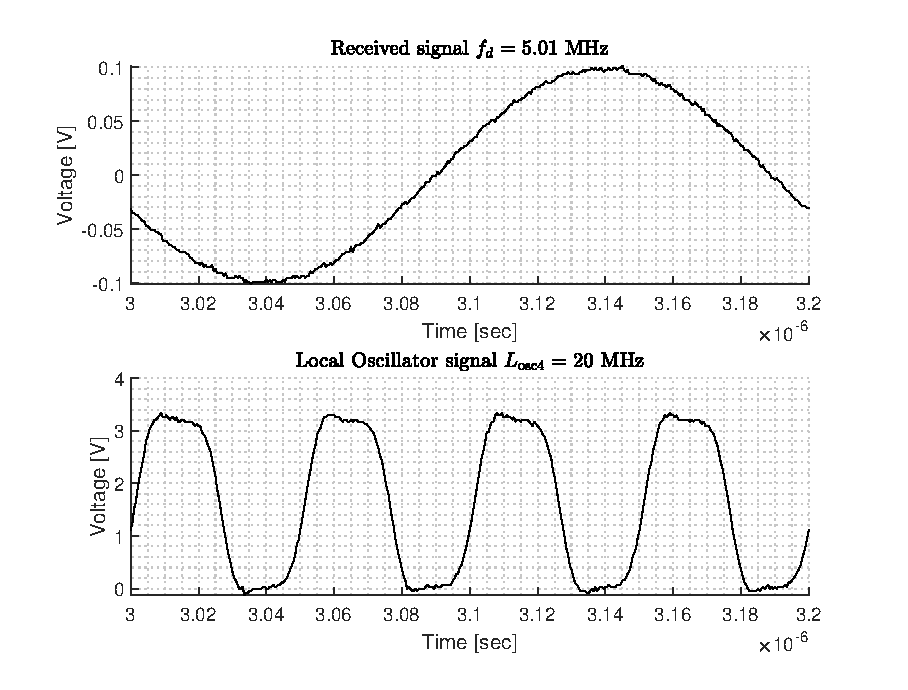
\includegraphics[width=.8\textwidth]{Figures/4_demod_pcb_in.eps}
	\caption[Measured input of demodulator PCB]{Measured input of demodulator PCB (Above) Input from received signal (Below) Input from local oscillator ($f_{0}\cdot4$)}
	\label{fig:4_demod_in}
\end{figure}
\begin{figure}[htbp]
	\centering
	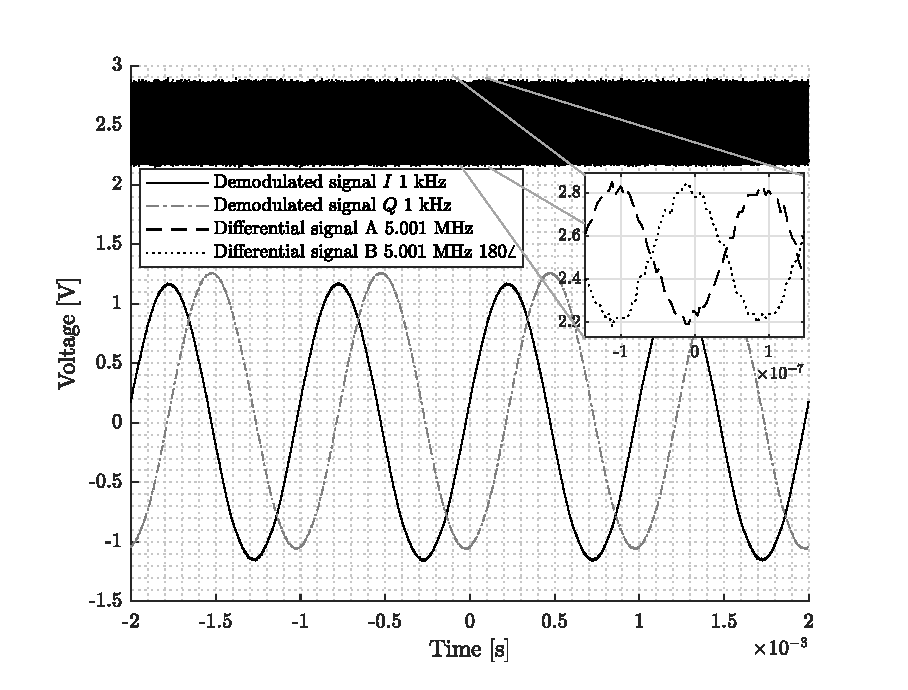
\includegraphics[width=.8\textwidth]{Figures/4_demod_pcb_out.eps}
	\caption[Measured output of demodulator PCB]{Measured output of demodulator PCB}
	\label{fig:4_demod_out}
\end{figure}

\subsection{Sample and Hold Amplifier}
Seen in \cref{fig:4_sample_hold_pcb} is the measured inputs and outputs of the circuit during the experiment. Above is the I-Q input and in the middle is the sample gating, and below is the output signal. On the output signal, it is noted the corresponding voltage transients for every pulse in the gate input.
\begin{figure}[htbp]
	\centering
	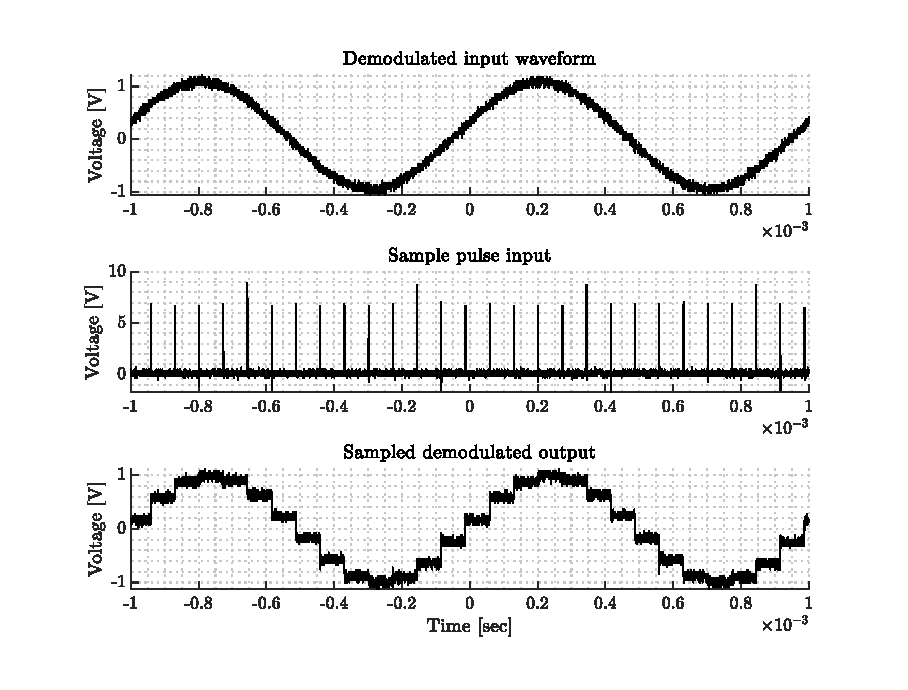
\includegraphics[width=.8\textwidth]{Figures/4_sampler_pcb.eps}
	\caption{Measured input and output of Sample and Hold amplifier}
	\label{fig:4_sample_hold_pcb}
\end{figure}

\subsection{Active Filter}
\begin{figure}
	\centering
	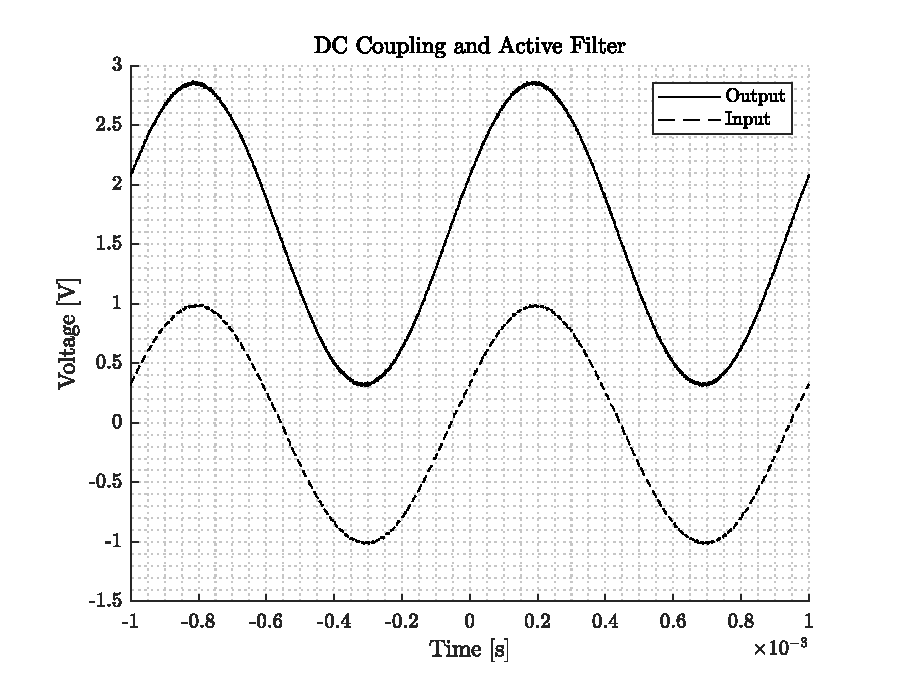
\includegraphics[width=.8\textwidth]{Figures/5_dccoupler_filter_measurement.eps}
	\caption{Measured input and output of Active filter and DC Coupler}
	\label{fig:5_dccoupler_measured}
\end{figure}
A \qty{1}{\kilo\hertz} input signal is received on the input SMA connector from a function generator and probed with an oscilloscope. $\pm\qty{5}{\volt}$ is supplied to the power terminals. Next, the output SMA connector is probed with an oscilloscope and the data is recorded. The dashed line is the \gls{ac} coupled input signal with \qty{1}{\volt} amplitude and the solid line is the amplified \gls{dc} coupled output signal. Seen in \cref{fig:5_dccoupler_measured} is the measured input and output of the DC coupler and active filter. This measurement confirms its operation as expected when comparing to the simulation shown earlier in the report.

\subsection{Digital Signal Processor}

\begin{figure}[htbp]
	\centering
	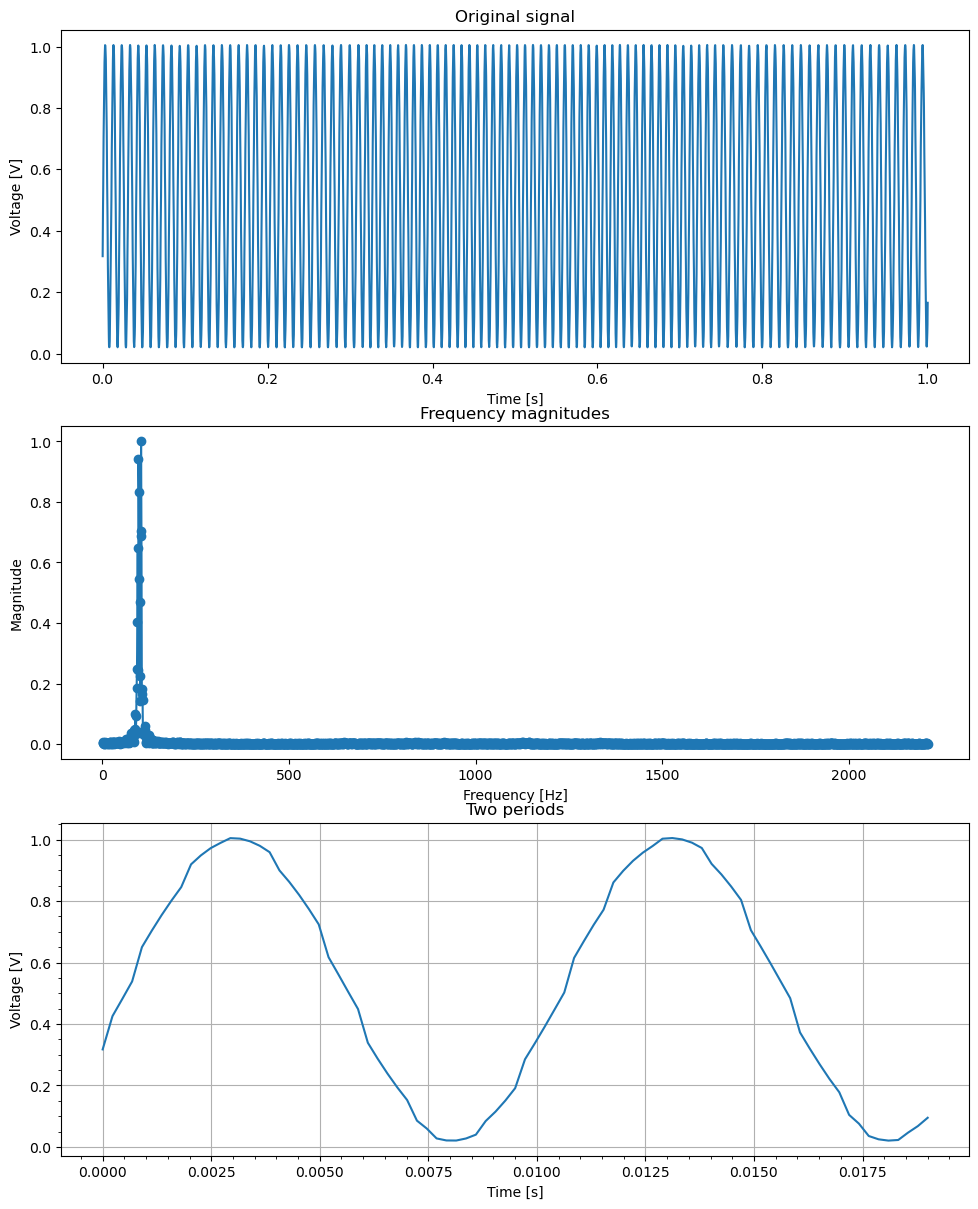
\includegraphics[width=.8\textwidth]{Figures/5_velocity_estimation_output.png}
	\caption{Velocity estimation with XADC and Jupyter}
	\label{fig:5_velocity_estimation_output}
\end{figure}

\begin{figure}[htbp]
	\centering
	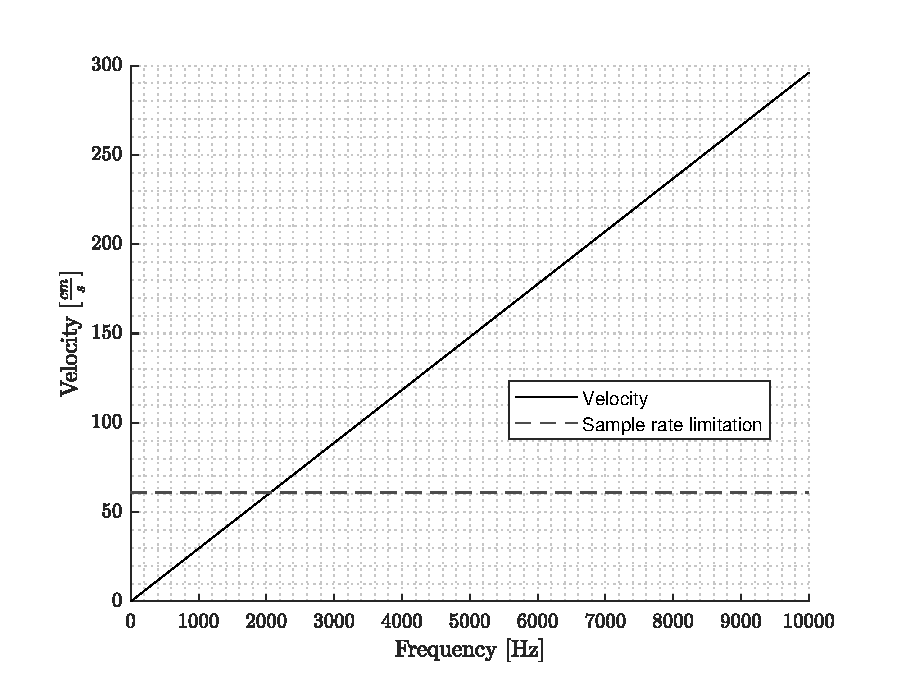
\includegraphics[width=.8\textwidth]{Figures/5_velocity_estimation_limit.eps}
	\caption{Velocity estimator with sample rate limitation}
	\label{fig:5_dsp_samplerate_limit}
\end{figure}

\section{Pulse Generator and Power Stage}
Using the pulse generator and the power stage, an experiment is performed where the complementary PWM signals are generated and output to the gate driver of the power stage. In turn, the gate driver will drive the MOSFET pair and output a high-power output than the pulse generator can supply on its own through its \gls{gpio}.

\begin{figure}[htbp]
	\centering
	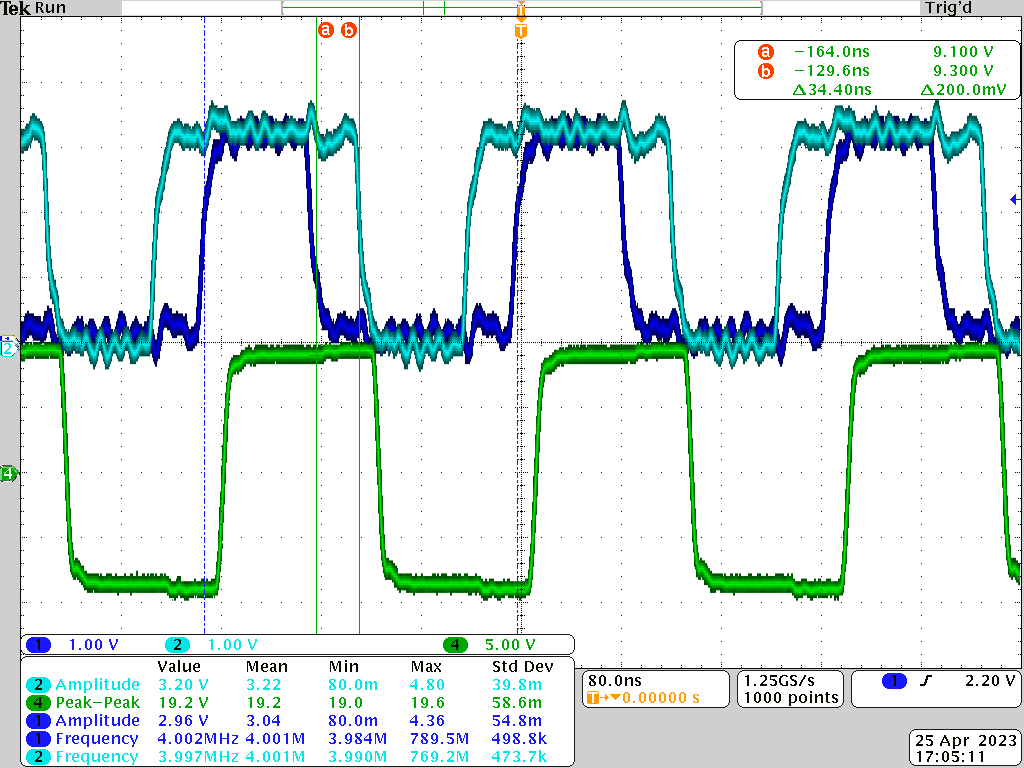
\includegraphics[width=.8\textwidth]{Figures/5_controlsystem_fpga_pwm.png}
	\caption{Complementary PWM output from the pulse generator and bipolar high power pulses}
	\label{fig:5_pulse_generator_experiment}
\end{figure}

Seen in \cref{fig:5_pulse_generator_experiment} are the measurements obtained from the pulse generator and power stage experiment. The measurements show the ability of the Pynq Z1 as a pulse generator is functioning as expected. As the power stage half-bridge is rail-to-rail, the output pulse voltages depend on the power supply voltage. In this case, the experiment is using a \qty{30}{\volt} maximum \gls{dcps}, and the output peak pulse voltages are $\pm \qty{30}{\volt}$. However, the power stage itself is specified for bipolar operating voltages up to $\pm \qty{100}{\volt}$, or unipolar voltages $\pm \qty{200}{\volt}$.

\section{Doppler String Phantom Experiment}
\begin{figure}[htbp]
	\centering
	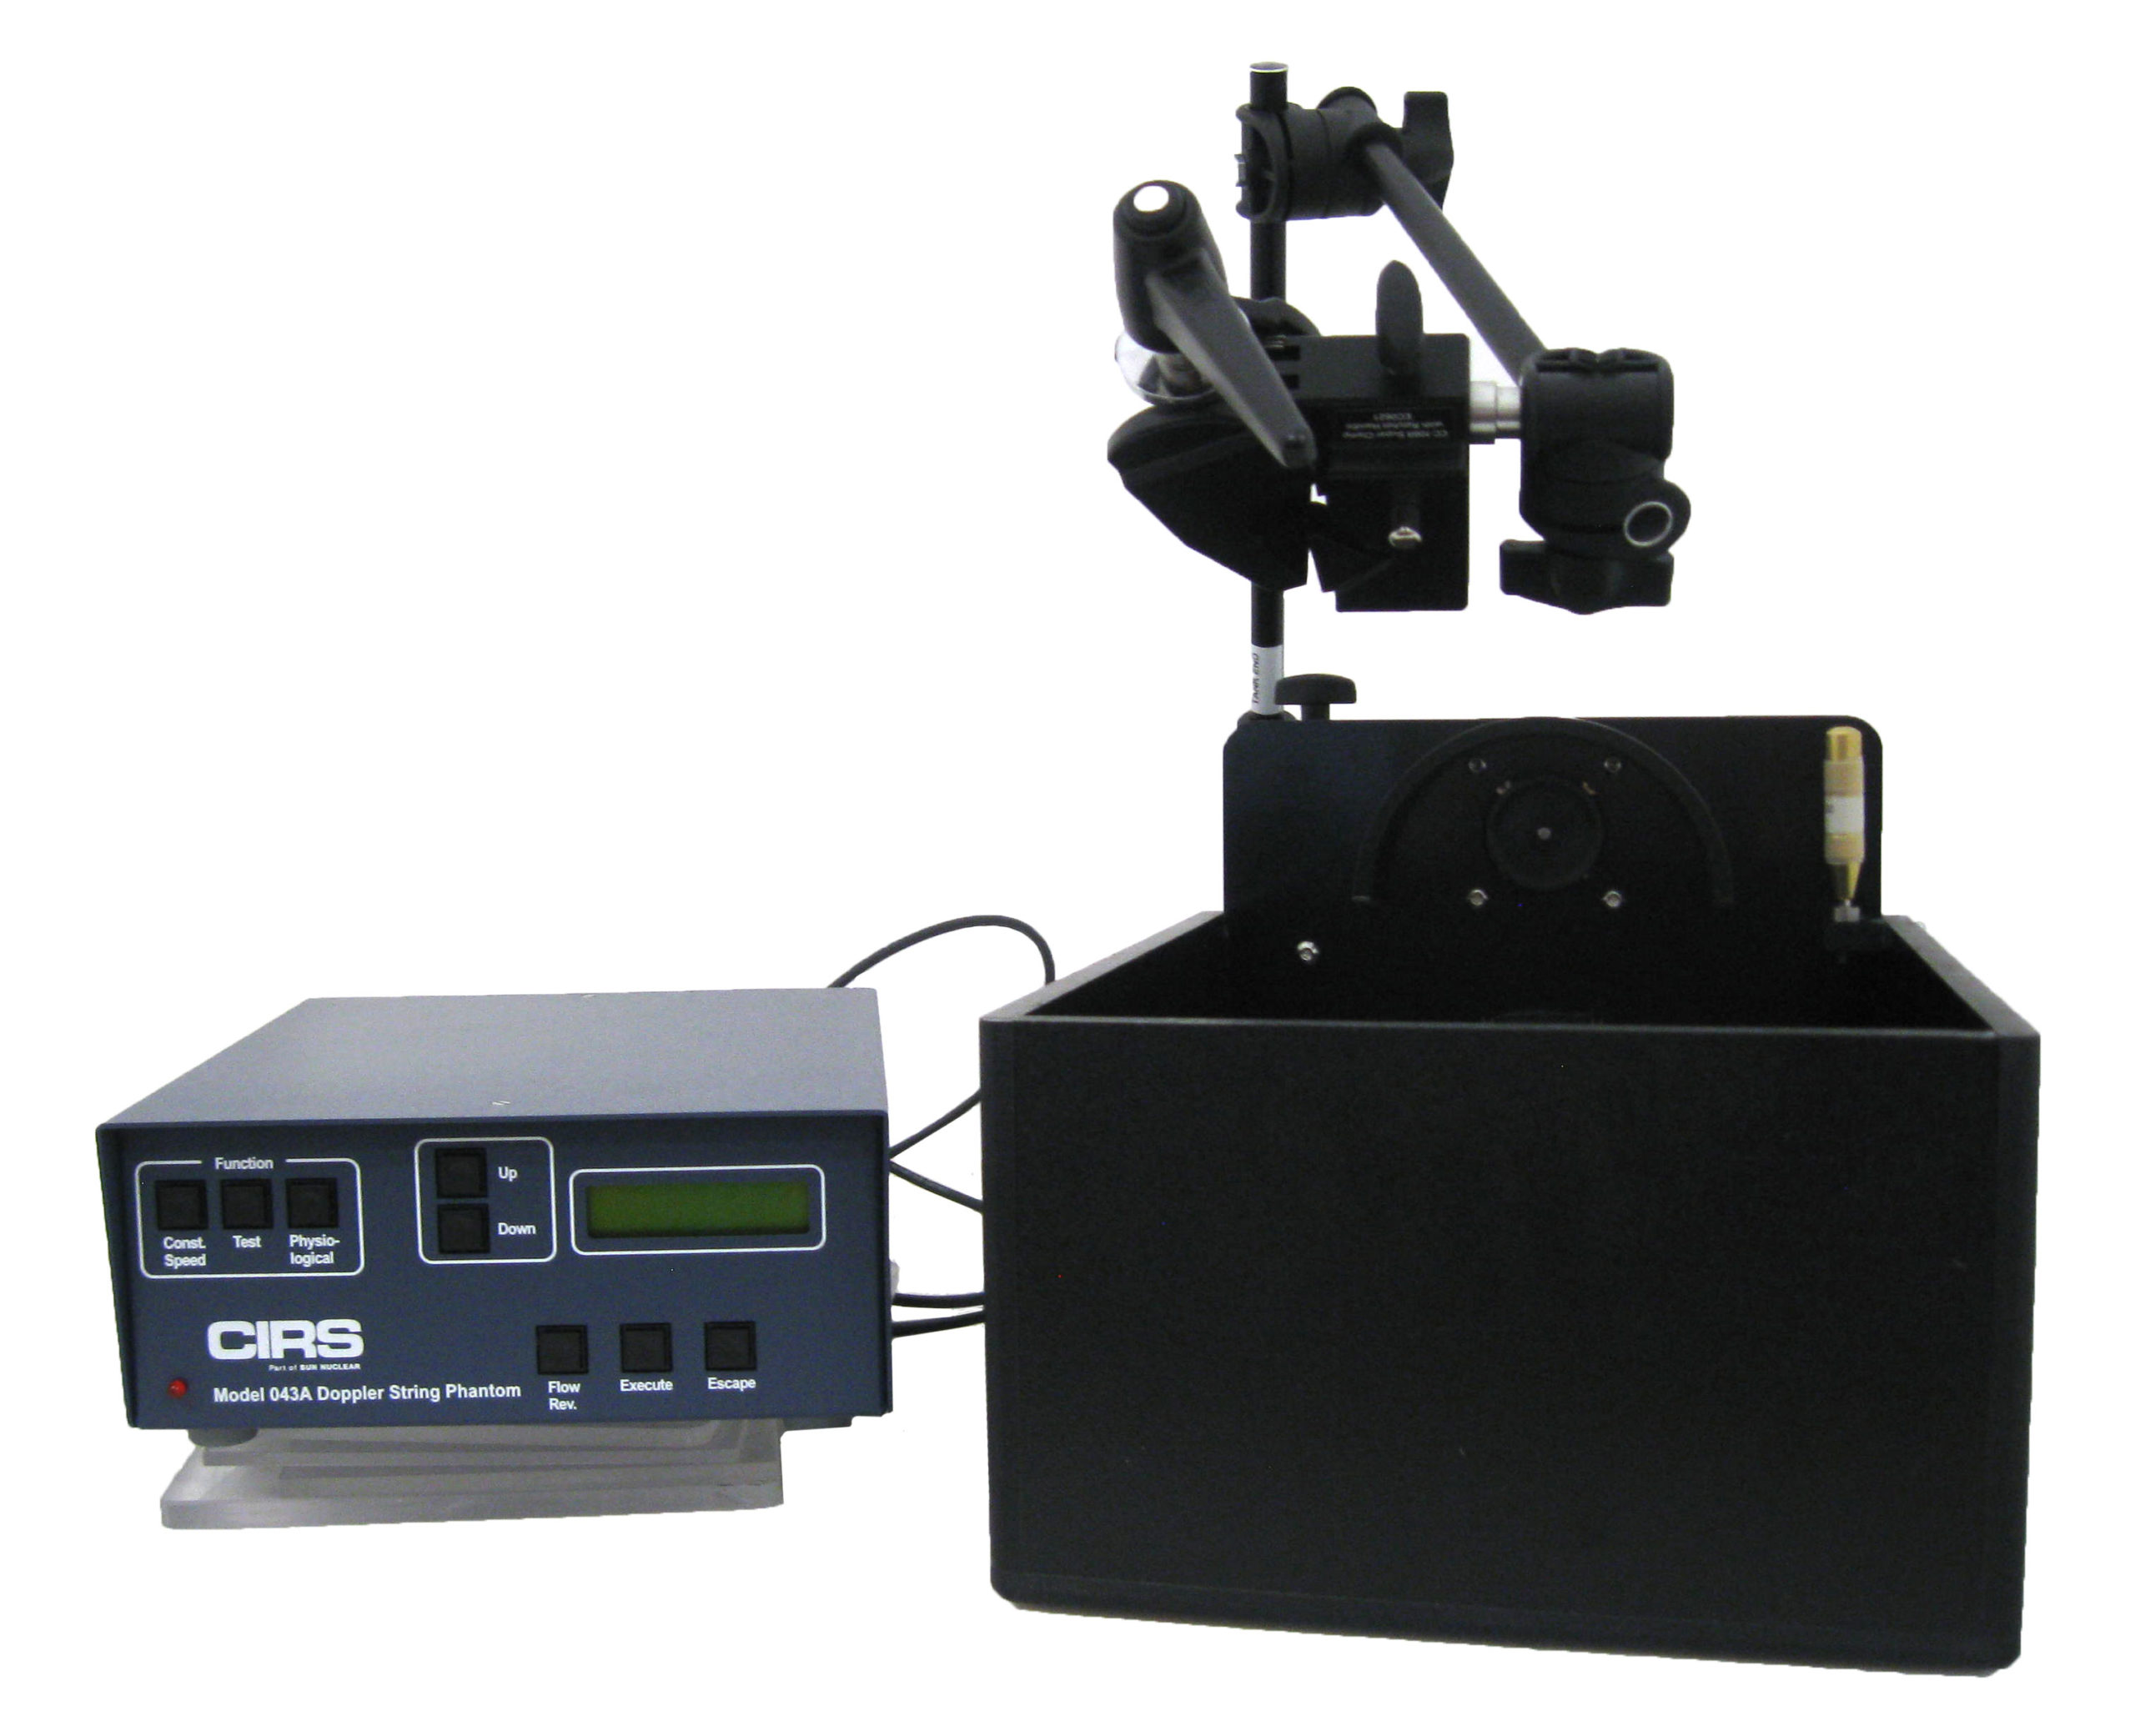
\includegraphics[width=.8\textwidth]{Figures/5_cirs_043a_image.jpg}
	\caption[CIRS Model 043A Doppler String Phantom]{CIRS Model 043A Doppler String Phantom with (left) motor controller and (right) tank and string loop}
	\label{fig:5_doppler_string_phantom}
\end{figure}
Seen in \cref{fig:5_doppler_string_phantom} is the CIRS A043 Doppler String Phantom is a device used to evaluate the performance of Doppler ultrasound imaging systems. The phantom consists of a string that is driven by a motor. The motor can be programmed to move at different speeds and directions, and can also be configured to drive the string with physiological waveforms, such as a carotid artery for validation purposes. A Doppler string phantom validation technique is widely used in research, development, and quality assurance of Doppler ultrasound equipment.
\begin{figure}[htbp]
	\centering
%	\begin{adjustbox}{width=\textwidth}%
%		

\tikzset{every picture/.style={line width=0.75pt}} %set default line width to 0.75pt

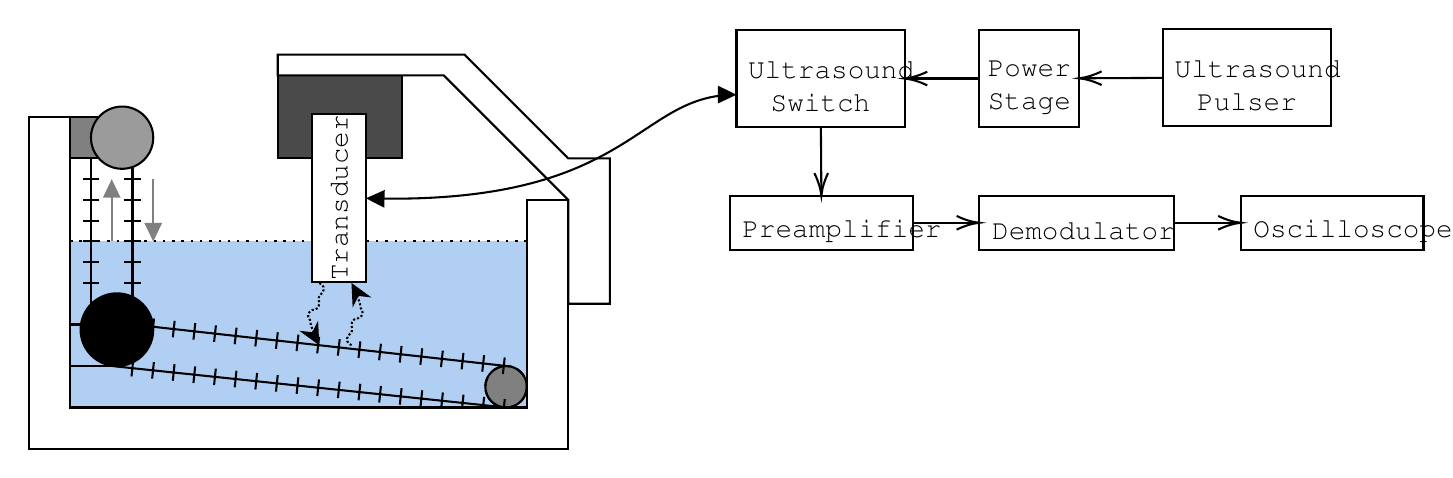
\begin{tikzpicture}[x=0.75pt,y=0.75pt,yscale=-1,xscale=1]
	%uncomment if require: \path (0,244); %set diagram left start at 0, and has height of 244

	%Shape: Rectangle [id:dp6722494395467095]
	\draw  [fill={rgb, 255:red, 74; green, 144; blue, 226 }  ,fill opacity=0.43 ][dash pattern={on 0.84pt off 2.51pt}] (40,120) -- (260,120) -- (260,200) -- (40,200) -- cycle ;
	%Shape: Rectangle [id:dp07000140128396126]
	\draw  [fill={rgb, 255:red, 74; green, 74; blue, 74 }  ,fill opacity=1 ] (140,40) -- (200,40) -- (200,80) -- (140,80) -- cycle ;
	%Shape: Circle [id:dp1435775000611489]
	\draw  [fill={rgb, 255:red, 128; green, 128; blue, 128 }  ,fill opacity=1 ] (240,190) .. controls (240,184.48) and (244.48,180) .. (250,180) .. controls (255.52,180) and (260,184.48) .. (260,190) .. controls (260,195.52) and (255.52,200) .. (250,200) .. controls (244.48,200) and (240,195.52) .. (240,190) -- cycle ;
	%Straight Lines [id:da5994952267655665]
	\draw    (50,70) -- (50,150) (54,80) -- (46,80)(54,90) -- (46,90)(54,100) -- (46,100)(54,110) -- (46,110)(54,120) -- (46,120)(54,130) -- (46,130)(54,140) -- (46,140) ;
	%Shape: Rectangle [id:dp7130303275600529]
	\draw  [color={rgb, 255:red, 0; green, 0; blue, 0 }  ,draw opacity=1 ][fill={rgb, 255:red, 128; green, 128; blue, 128 }  ,fill opacity=1 ] (40,60) -- (60,60) -- (60,80) -- (40,80) -- cycle ;
	%Shape: Circle [id:dp883251536454338]
	\draw  [fill={rgb, 255:red, 0; green, 0; blue, 0 }  ,fill opacity=1 ] (45,162.5) .. controls (45,152.84) and (52.84,145) .. (62.5,145) .. controls (72.16,145) and (80,152.84) .. (80,162.5) .. controls (80,172.16) and (72.16,180) .. (62.5,180) .. controls (52.84,180) and (45,172.16) .. (45,162.5) -- cycle ;
	%Shape: Rectangle [id:dp3769942512437483]
	\draw   (40,160) -- (60,160) -- (60,180) -- (40,180) -- cycle ;
	%Shape: Circle [id:dp8079321779320666]
	\draw  [dash pattern={on 3.75pt off 3pt on 7.5pt off 1.5pt}] (240,190) .. controls (240,184.48) and (244.48,180) .. (250,180) .. controls (255.52,180) and (260,184.48) .. (260,190) .. controls (260,195.52) and (255.52,200) .. (250,200) .. controls (244.48,200) and (240,195.52) .. (240,190) -- cycle ;
	%Straight Lines [id:da7273832971820673]
	\draw    (60,180) -- (250,200) (70.36,177.07) -- (69.53,185.02)(80.31,178.12) -- (79.47,186.07)(90.25,179.16) -- (89.42,187.12)(100.2,180.21) -- (99.36,188.17)(110.14,181.26) -- (109.31,189.21)(120.09,182.3) -- (119.25,190.26)(130.03,183.35) -- (129.2,191.31)(139.98,184.4) -- (139.14,192.35)(149.92,185.44) -- (149.09,193.4)(159.87,186.49) -- (159.03,194.45)(169.81,187.54) -- (168.98,195.49)(179.76,188.58) -- (178.92,196.54)(189.7,189.63) -- (188.87,197.59)(199.65,190.68) -- (198.81,198.63)(209.59,191.72) -- (208.76,199.68)(219.54,192.77) -- (218.7,200.73)(229.48,193.82) -- (228.65,201.77)(239.43,194.87) -- (238.59,202.82)(249.37,195.91) -- (248.54,203.87) ;
	%Straight Lines [id:da05910308874228931]
	\draw    (70,160) -- (250,180) (80.38,157.13) -- (79.5,165.08)(90.32,158.23) -- (89.44,166.18)(100.26,159.34) -- (99.37,167.29)(110.2,160.44) -- (109.31,168.39)(120.14,161.55) -- (119.25,169.5)(130.07,162.65) -- (129.19,170.6)(140.01,163.75) -- (139.13,171.71)(149.95,164.86) -- (149.07,172.81)(159.89,165.96) -- (159.01,173.91)(169.83,167.07) -- (168.95,175.02)(179.77,168.17) -- (178.89,176.12)(189.71,169.28) -- (188.82,177.23)(199.65,170.38) -- (198.76,178.33)(209.59,171.48) -- (208.7,179.44)(219.52,172.59) -- (218.64,180.54)(229.46,173.69) -- (228.58,181.64)(239.4,174.8) -- (238.52,182.75)(249.34,175.9) -- (248.46,183.85) ;
	%Straight Lines [id:da12196496059097228]
	\draw [fill={rgb, 255:red, 0; green, 0; blue, 0 }  ,fill opacity=1 ]   (70,70) -- (70,160) (74,80) -- (66,80)(74,90) -- (66,90)(74,100) -- (66,100)(74,110) -- (66,110)(74,120) -- (66,120)(74,130) -- (66,130)(74,140) -- (66,140)(74,150) -- (66,150) ;
	%Curve Lines [id:da7394389878662597]
	\draw  [dash pattern={on 0.75pt off 0.75pt}]  (160,140) .. controls (162.22,141.07) and (162.72,142.66) .. (161.49,144.77) .. controls (159.76,145.92) and (159.25,147.46) .. (159.97,149.41) .. controls (159.98,151.75) and (158.86,152.97) .. (156.59,153.07) .. controls (154.34,154.26) and (153.98,155.87) .. (155.53,157.88) -- (155.94,160.34) -- (158.75,167.6) ;
	\draw [shift={(160,170)}, rotate = 241.56] [fill={rgb, 255:red, 0; green, 0; blue, 0 }  ][line width=0.08]  [draw opacity=0] (10.72,-5.15) -- (0,0) -- (10.72,5.15) -- (7.12,0) -- cycle    ;
	%Curve Lines [id:da9786153302440782]
	\draw  [dash pattern={on 0.75pt off 0.75pt}]  (175.5,170) .. controls (173.28,168.93) and (172.78,167.34) .. (174,165.23) .. controls (175.74,164.08) and (176.25,162.54) .. (175.53,160.59) .. controls (175.52,158.25) and (176.64,157.03) .. (178.91,156.93) .. controls (181.16,155.74) and (181.51,154.13) .. (179.97,152.12) -- (179.56,149.66) -- (176.74,142.4) ;
	\draw [shift={(175.5,140)}, rotate = 61.56] [fill={rgb, 255:red, 0; green, 0; blue, 0 }  ][line width=0.08]  [draw opacity=0] (10.72,-5.15) -- (0,0) -- (10.72,5.15) -- (7.12,0) -- cycle    ;
	%Straight Lines [id:da7205891380538312]
	\draw [color={rgb, 255:red, 128; green, 128; blue, 128 }  ,draw opacity=1 ]   (80,90) -- (80,117) ;
	\draw [shift={(80,120)}, rotate = 270] [fill={rgb, 255:red, 128; green, 128; blue, 128 }  ,fill opacity=1 ][line width=0.08]  [draw opacity=0] (8.93,-4.29) -- (0,0) -- (8.93,4.29) -- cycle    ;
	%Straight Lines [id:da631680111682684]
	\draw [color={rgb, 255:red, 128; green, 128; blue, 128 }  ,draw opacity=1 ]   (60,93) -- (60,120) ;
	\draw [shift={(60,90)}, rotate = 90] [fill={rgb, 255:red, 128; green, 128; blue, 128 }  ,fill opacity=1 ][line width=0.08]  [draw opacity=0] (8.93,-4.29) -- (0,0) -- (8.93,4.29) -- cycle    ;
	%Shape: Polygon [id:ds5396773368746502]
	\draw  [fill={rgb, 255:red, 255; green, 255; blue, 255 }  ,fill opacity=1 ] (40,60) -- (40,200) -- (260,200) -- (260,100) -- (280,100) -- (280,220) -- (20,220) -- (20,60) -- cycle ;
	%Shape: Circle [id:dp9531409722820131]
	\draw  [fill={rgb, 255:red, 155; green, 155; blue, 155 }  ,fill opacity=1 ] (50,70) .. controls (50,61.72) and (56.72,55) .. (65,55) .. controls (73.28,55) and (80,61.72) .. (80,70) .. controls (80,78.28) and (73.28,85) .. (65,85) .. controls (56.72,85) and (50,78.28) .. (50,70) -- cycle ;
	%Straight Lines [id:da9454073791401769]
	\draw [fill={rgb, 255:red, 255; green, 255; blue, 255 }  ,fill opacity=1 ]   (280,150) -- (280,100) -- (220,40) -- (140,40) -- (140,30) -- (230,30) -- (280,80) -- (300,80) -- (300,150) -- cycle ;

	% Text Node
	\draw  [fill={rgb, 255:red, 255; green, 255; blue, 255 }  ,fill opacity=1 ]  (156.5,58.5) -- (182.5,58.5) -- (182.5,139.5) -- (156.5,139.5) -- cycle  ;
	\draw (169.5,99) node  [rotate=-270] [align=left] {{\fontfamily{pcr}\selectfont Transducer}};
	% Text Node
	\draw  [fill={rgb, 255:red, 255; green, 255; blue, 255 }  ,fill opacity=1 ]  (361,18) -- (442,18) -- (442,65) -- (361,65) -- cycle  ;
	\draw (401.5,41.5) node   [align=left] {\begin{minipage}[lt]{52.33pt}\setlength\topsep{0pt}
			\begin{center}
				{\fontfamily{pcr}\selectfont Ultrasound}\\{\fontfamily{pcr}\selectfont Switch}
			\end{center}

	\end{minipage}};
	% Text Node
	\draw  [fill={rgb, 255:red, 255; green, 255; blue, 255 }  ,fill opacity=1 ]  (478,18) -- (526,18) -- (526,65) -- (478,65) -- cycle  ;
	\draw (502,41.5) node   [align=left] {\begin{minipage}[lt]{29.8pt}\setlength\topsep{0pt}
			\begin{center}
				{\fontfamily{pcr}\selectfont Power}\\{\fontfamily{pcr}\selectfont Stage}
			\end{center}

	\end{minipage}};
	% Text Node
	\draw  [fill={rgb, 255:red, 255; green, 255; blue, 255 }  ,fill opacity=1 ]  (566.5,17.5) -- (647.5,17.5) -- (647.5,64.5) -- (566.5,64.5) -- cycle  ;
	\draw (607,41) node   [align=left] {\begin{minipage}[lt]{52.33pt}\setlength\topsep{0pt}
			\begin{center}
				{\fontfamily{pcr}\selectfont Ultrasound}\\{\fontfamily{pcr}\selectfont Pulser}
			\end{center}

	\end{minipage}};
	% Text Node
	\draw  [fill={rgb, 255:red, 255; green, 255; blue, 255 }  ,fill opacity=1 ]  (358,98) -- (446,98) -- (446,124) -- (358,124) -- cycle  ;
	\draw (402,111) node   [align=left] {\begin{minipage}[lt]{57.26pt}\setlength\topsep{0pt}
			\begin{center}
				{\fontfamily{pcr}\selectfont Preamplifier}
			\end{center}

	\end{minipage}};
	% Text Node
	\draw  [fill={rgb, 255:red, 255; green, 255; blue, 255 }  ,fill opacity=1 ]  (478,98) -- (572,98) -- (572,124) -- (478,124) -- cycle  ;
	\draw (525,111) node   [align=left] {\begin{minipage}[lt]{61.2pt}\setlength\topsep{0pt}
			\begin{center}
				{\fontfamily{pcr}\selectfont Demodulator}
			\end{center}

	\end{minipage}};
	% Text Node
	\draw  [fill={rgb, 255:red, 255; green, 255; blue, 255 }  ,fill opacity=1 ]  (604,98) -- (692,98) -- (692,124) -- (604,124) -- cycle  ;
	\draw (648,111) node   [align=left] {\begin{minipage}[lt]{56.9pt}\setlength\topsep{0pt}
			\begin{center}
				{\fontfamily{pcr}\selectfont Oscilloscope}
			\end{center}

	\end{minipage}};
	% Connection
	\draw    (478,41.5) -- (444,41.5) ;
	\draw [shift={(442,41.5)}, rotate = 360] [color={rgb, 255:red, 0; green, 0; blue, 0 }  ][line width=0.75]    (10.93,-3.29) .. controls (6.95,-1.4) and (3.31,-0.3) .. (0,0) .. controls (3.31,0.3) and (6.95,1.4) .. (10.93,3.29)   ;
	% Connection
	\draw    (566.5,41.19) -- (528,41.38) ;
	\draw [shift={(526,41.39)}, rotate = 359.73] [color={rgb, 255:red, 0; green, 0; blue, 0 }  ][line width=0.75]    (10.93,-3.29) .. controls (6.95,-1.4) and (3.31,-0.3) .. (0,0) .. controls (3.31,0.3) and (6.95,1.4) .. (10.93,3.29)   ;
	% Connection
	\draw    (401.67,65) -- (401.89,96) ;
	\draw [shift={(401.91,98)}, rotate = 269.59] [color={rgb, 255:red, 0; green, 0; blue, 0 }  ][line width=0.75]    (10.93,-3.29) .. controls (6.95,-1.4) and (3.31,-0.3) .. (0,0) .. controls (3.31,0.3) and (6.95,1.4) .. (10.93,3.29)   ;
	% Connection
	\draw    (446,111) -- (476,111) ;
	\draw [shift={(478,111)}, rotate = 180] [color={rgb, 255:red, 0; green, 0; blue, 0 }  ][line width=0.75]    (10.93,-3.29) .. controls (6.95,-1.4) and (3.31,-0.3) .. (0,0) .. controls (3.31,0.3) and (6.95,1.4) .. (10.93,3.29)   ;
	% Connection
	\draw    (572,111) -- (602,111) ;
	\draw [shift={(604,111)}, rotate = 180] [color={rgb, 255:red, 0; green, 0; blue, 0 }  ][line width=0.75]    (10.93,-3.29) .. controls (6.95,-1.4) and (3.31,-0.3) .. (0,0) .. controls (3.31,0.3) and (6.95,1.4) .. (10.93,3.29)   ;
	% Connection
	\draw    (357.41,49.38) .. controls (312.15,51.65) and (308.79,102.38) .. (184.38,99.26) ;
	\draw [shift={(182.5,99.21)}, rotate = 1.67] [fill={rgb, 255:red, 0; green, 0; blue, 0 }  ][line width=0.08]  [draw opacity=0] (8.93,-4.29) -- (0,0) -- (8.93,4.29) -- cycle    ;
	\draw [shift={(361,49.3)}, rotate = 180.36] [fill={rgb, 255:red, 0; green, 0; blue, 0 }  ][line width=0.08]  [draw opacity=0] (8.93,-4.29) -- (0,0) -- (8.93,4.29) -- cycle    ;

\end{tikzpicture}

%	\end{adjustbox}%
	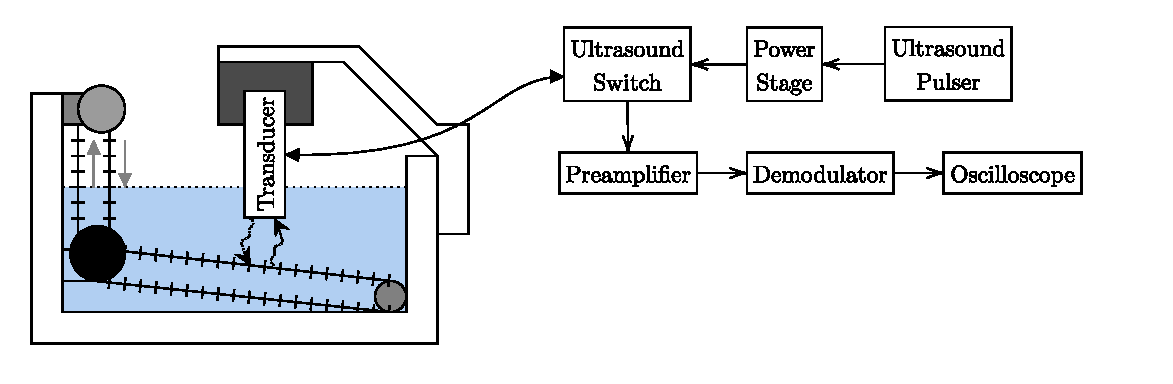
\includegraphics[width=\textwidth]{Figures/5_doppler_string_phantom_experiment.pdf}
	\caption{Doppler String Phantom experiment diagram (not to scale)}
	\label{fig:5_doppler_string_experiment}
\end{figure}
In \cref{fig:5_doppler_string_experiment} is a diagram of the experiment to be performed with the analogue front-end to evaluate the performance of the system. The ultrasound system is being controlled by the ultrasound pulser running on the PYNQ-Z1 board. The transducer used in the experiment is a piezoelectric \qty{5}{\mega\hertz} commercial transducer. The entire system operates at a \texttt{PRF} frequency of \qty{15}{\kilo\hertz}. First, the string is mounted in the string phantom loop. Next, the transducer is mounted on a movable arm and submerged in the water. When the ultrasound waves strike the moving string, the frequency of the reflected waves is shifted due to the Doppler effect. This frequency shift provides information about the velocity and direction of the simulated blood flow. Here, the ultrasound system measures the frequency shift and this can in turn be calculated into a velocity. This data can be analyzed to assess the accuracy and performance of the Doppler ultrasound system. The phantom allows for calibration of the system and evaluation of factors such as velocity sensitivity, and spectral Doppler analysis when looking at the \gls{psd} over time. Unfortunately, when conducting the experiment, a design review indicated that the pulser required a modification to the output of the power stage to ensure the potential across the transducer is bled off during rest. However, this must be carefully balanced to ensure that an increased load is not attenuating the received signal. Two solutions were proposed:
\begin{enumerate}
	\item A resistor to reference voltage in parallel with the transducer
	\item A second ultrasound switch, functionally inverse of the primary ultrasound switch to ensure received signal does not get attenuated by pulser circuit
\end{enumerate}